
\chapter{Permian Basin Background}
\label{CHAP:3}



In this chapter, we review the scientific background of the induced seismicity problem.
We describe the geodetic datasets available to study the problem, and we present strategies and challenges for processing Sentinel-1 InSAR data over West Texas. We demonstrate that tropospheric noise is the dominant InSAR noise source.


\section{Shale Development and Induced Seismicity}
\label{sec:ch3-oil}

Texas has been a leading producer of oil and gas for over a century \citep{Frohlich2016HistoricalReviewInduced, TheAcademyofMedicine2017EnvironmentalCommunityImpacts}. It became the nation's largest producer of crude oil after the first successful vertical well was drilled south of Beaumont, TX in 1901. These ``conventional'' wells were the primary mode of production in multiple oil fields across the state. It wasn't until the early 2000s that advances in horizontal drilling and hydraulic fracturing (also known as fracking, Figure \ref{fig:ch3-oil-drilling}) opened up vast new shale resources which were previously unworkable \citep{Waters2006Spe103202Ms}. 
For example, the Wolfcamp shale in Texas' Permian Basin is the largest continuous oil field that has ever been discovered in the United States, containing 20 billion barrels of oil and 16 trillion cubic feet of gas \citep{Gaswirth2016AssessmentUndiscoveredContinuous}. While areas of the Wolfcamp shale in the Midland Basin have been traditionally developed using vertical wells, the ability to extend subsurface drilling horizontally (Figure \ref{fig:ch3-oil-drilling}b) and increase production using enhanced oil recovery (EOR, Figure \ref{fig:ch3-oil-drilling}d)
allowed many new areas to be economically viable for oil and gas production (Figure \ref{fig:ch3-drilling-pads}).


%Figure \ref{fig:oil-drilling} shows a simplified diagram of the operation techniques of horizontal drilling, hydraulic fracturing, wastewater disposal, and enhanced oil recovery.
%These shale resources are also known as ``tight oil` and ``shale gas'', and may collectively be referred to as ``unconventional''. 


\begin{figure}
	\centering
%	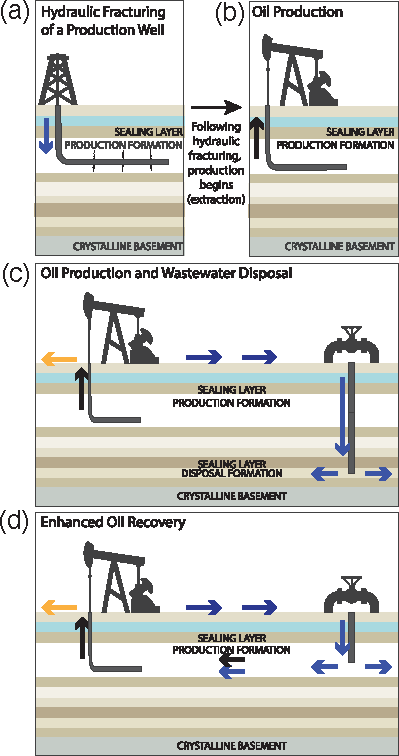
\includegraphics[width=0.6\linewidth]{figures/chapter3-permian/oil-page.pdf}
	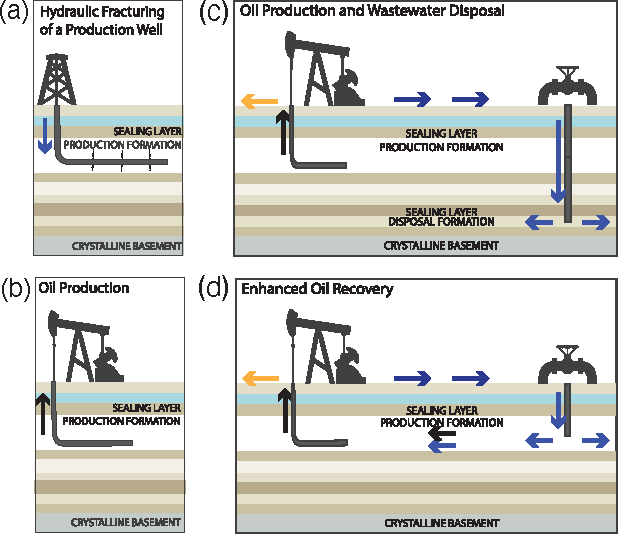
\includegraphics[width=\linewidth]{figures/chapter3-permian/oil-page-square.pdf}
	\caption[Diagram of unconventional oil production operations]{
		Simplified diagrams of oil-field operations. Arrows show the directions of fluid being injected or withdrawn. Arrow color indicates the contents of the fluid: black (oil, gas, and wastewater), yellow (oil and gas), and blue (wastewater). 
		(a) In a hydraulic fracturing operation, fluids are injected at high pressure into a production well, causing fractures in the surrounding rock that increase permeability. Increased permeability allows the extraction of oil or gas from a larger region. Following the hydraulic fracturing of a well, the well goes into production (b). 
		(c) Production wells extract oil and gas, and as a byproduct, salt water (commonly called ``produced water'' or ``wastewater''), which is injected to a different subsurface formation at a disposal well. 
		(d) Enhanced oil recovery (EOR), an alternative to wastewater disposal, involves injecting the water back into the formation holding the oil and gas to sweep oil and gas toward the production well.
		(Figure adapted from \citep{Rubinstein2015MythsFactsWastewater})
	}
	\label{fig:ch3-oil-drilling}
\end{figure}

%This report uses the term “shale” to describe organic rich formations containing natural gas (shale gas) and/or oil (tight oil) that require multiple hydraulic fractures, usually created from long wells drilled horizontally, to produce hydrocarbons profitablyThe term “tight oil” may include hybrid formations containing oil that has migrated into very tight rock. Many experts refer to shale gas and tight oil resources collectively as “unconventional.” \cite{TheAcademyofMedicine2017EnvironmentalCommunityImpacts}
%lthough these resources have been known to exist for decades, rapid expansion of oil and gas production from shale formations was made possible by the innovative combined use of two technologies—hydraulic fracturing (referred to colloquially as “fracking”) and horizontal drilling.


\begin{figure}
	\centering
	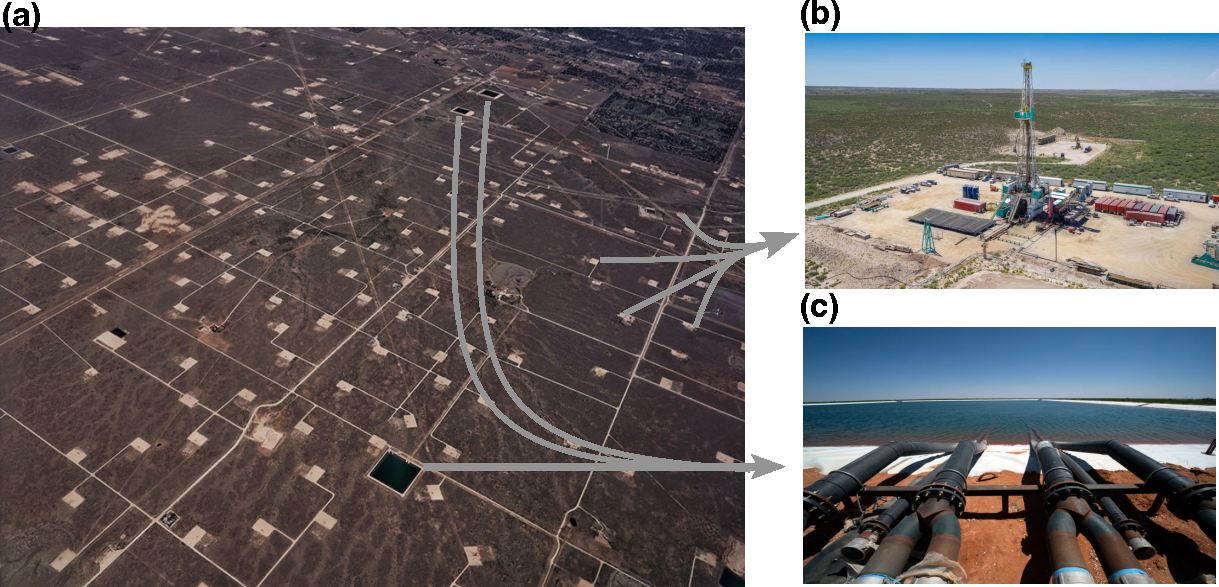
\includegraphics[width=\linewidth]{figures/chapter3-permian/permian-images.pdf}
	\caption[Permian Basin drilling pads]{
		(a) Aerial view of drilling pads throughout the Permian Basin
		(b) Drilling rig set up on one pad
		(Source: XTO Energy)
		(c) Water condensate pit used to store fresh water condensed from natural gas or other flowback fluids (photo source: Benjamin Lowy)
	}
	\label{fig:ch3-drilling-pads}
\end{figure}


Despite the economic benefits that the new production technologies provided for Texas, concerns have been raised about possible environmental consequences of shale development \citep{TheAcademyofMedicine2017EnvironmentalCommunityImpacts, Scanlon2020WillWaterIssues}. 
%including injection of chemicals underground, water usage in semiarid areas and potential water contamination, and seismic activity
%For example, more than 30 billion bbl of wastewater have been disposed throughout the Permian Basin \cite{Lemons2019SpatiotemporalStratigraphicTrends} and future Wolfcamp shale development is expected to generate $\sim$300 billion bbl of produced water \cite{Smye2021VariationsVerticalStress,  Scanlon2020WillWaterIssues}.
%Here we briefly review the  seismic activity induced from oil and gas production.
One concern is the triggering of seismic activity, as it has been recognized that injection or withdrawal of fluids from the subsurface can induce earthquakes along existing faults \citep{Ellsworth2013InjectionInducedEarthquakes, Simpson1988TwoTypesReservoir}.
Note that induced earthquakes are not limited to oil and gas operations \citep{Grigoli2017CurrentChallengesMonitoring, Foulger2018GlobalReviewHuman, Baan2017HumanInducedSeismicity}; they have also been associated with geothermal energy development \citep{Deichmann2009EarthquakesInducedStimulation}, mining operations \citep{Hasegawa1989InducedSeismicityMines}, water impoundment in reservoirs \citep{Talwani1997NatureReservoirInduced}, and CO$_2$ sequestration \citep{Gan2013GasInjectionMay}.



%2. Induced seismicity: historical in Texas
%3.  Why is it happening?
% Basic mechannisms of induced. pore pressure, mohr circle
% other methods to tie: spatio temporal linking. more plausible when there are many simultaneous factors



% 
%During this time period, an increase in low magnitude earthquakes was observed. While West Texas had few seismic monitoring stations set up, one array near Lajitas, TX had been operating since 2000 \citep{Frohlich2019OnsetCauseIncreased}.


\begin{figure}
	\centering
	%	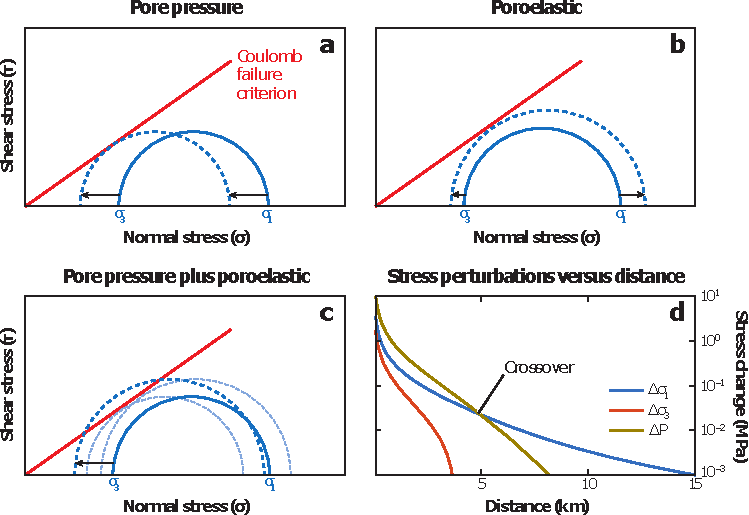
\includegraphics[width=\linewidth]{figures/chapter3-permian/mohr-circles.pdf}
	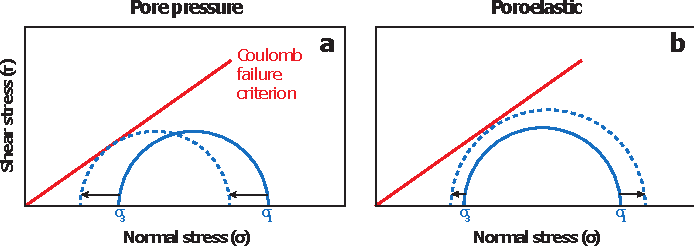
\includegraphics[width=\linewidth]{figures/chapter3-permian/mohr-circles-toponly.pdf}
	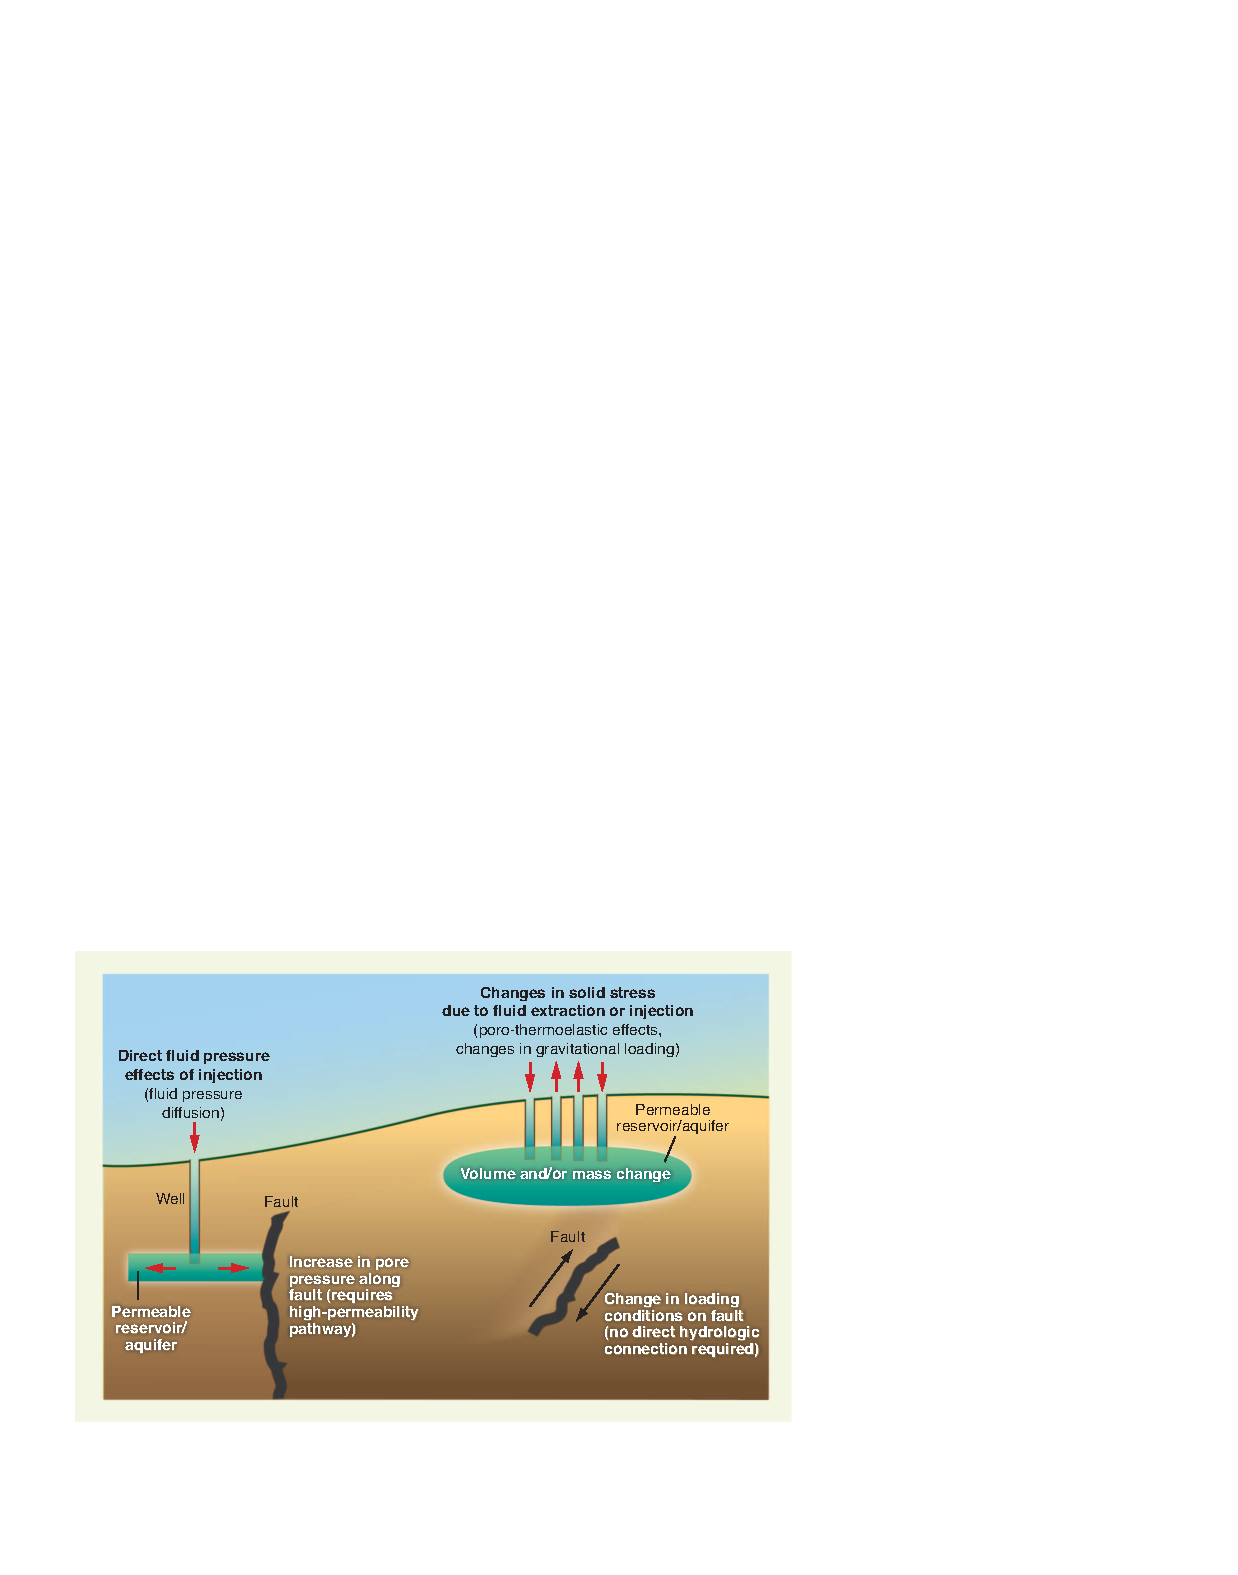
\includegraphics[width=\linewidth]{figures/chapter3-permian/injection-ellsworth.pdf}
	\caption[Effects of pore pressure perturbations and poroelastic stress changes on fault failure]{
		Effects of pore pressure perturbations and poroelastic stress changes on fault failure. Solid curves represent the initial stress state, and dashed curves represent the perturbed stress state. (a) Increased pore pressure reduces normal stress on the fault plane, moving the fault closer to the Coulomb failure criterion. (b) Poroelastic stresses increase differential stress. For both (a) and (b), pore pressure perturbations and stress changes, as well as the relative magnitude of changes, depend on parameters including time, distance, injection rate, diffusivity, and poroelastic parameters.
		(Bottom) Schematic diagram for each mechanism causing injection-induced earthquakes.
		(Top from \cite{Keranen2018InducedSeismicity}, bottom from \cite{Ellsworth2013InjectionInducedEarthquakes})
	}
	\label{fig:mohr-circles}
\end{figure}

One conceptual model for triggering earthquakes uses the Mohr-Coulomb failure criterion \citep{Hubbert1959RoleFluidPressure}.
The critical shear stress $\tau_{critical}$ required to promote fault slippage can be written as
\begin{equation}
\tau_{critical} = \tau_0 + \mu (\sigma_n - P)
\end{equation}
where $\tau_0$ is the cohesive strength of the sliding surface (often negligible), $\mu$ is the coefficient of friction, $\sigma_n$ is the normal stress, $P$ is the pore pressure \citep{Nicholson1990EarthquakeHazardAssociated, Ellsworth2013InjectionInducedEarthquakes}. Intuitively, increasing the shear stress or decreasing the normal stress ``unclamps'' the fault and encourages failure \citep{Shearer2019IntroductionSeismology}. Since increasing pore pressure lowers the effective normal stress, fluid injection can move critically stressed faults to failure and cause earthquakes (Figure \ref{fig:mohr-circles}a).
Alternatively, poroelastic effects from injection can change the loading conditions on a fault without a direct hydraulic connection, which can cause fault failure through increased differential stress (Figure \ref{fig:mohr-circles}b).

%This was determined to be the cause of many earthquakes in Oklahoma in 2014-2016 (cite). However, other causes may play a role in the Permian Basin earthquakes, including poroelastic effects that may be a factor 10s of kilometers away from injection, even without direct hydraulic connections \citep{Skoumal2020InducedSeismicityDelaware}


%Pressure from wastewater injection may play a role in certain areas (find that citation). This increasing of subsurface pore pressure could cause surface uplift in certain cases, and an example of this was reported on a single injection well (and single CO2 injection?) by \cite{Kim2018AssociationLocalizedGeohazards}.s



%Following \cite{Dahm2012RecommendationDiscriminationHuman}, we can classify these discrimination methodsin three main families: physics-based methods, statistics-based methods, and source parameters-basedmethods




In Texas, earthquakes have occurred in close association with petroleum activities since 1925, but the rate of earthquakes in the last decade has increased over tenfold \citep{Frohlich2016HistoricalReviewInduced, Skoumal2020InducedSeismicityDelaware}.
To better understand the causes of these earthquakes and to assess the likelihood of infrastructure damage, 
the State of Texas funded the Texas Seismological Network (TexNet) to record earthquakes down to M2.0 across the state starting in 2017 \citep{Savvaidis2019TexnetStatewideSeismological}. 
By that time, there were over 130,000 active production wells, 23,000 active EOR wells, and nearly 3800 active saltwater disposal (SWD) wells in the Permian Basin (Figure \ref{fig:permian-oil-6panel} (a)).  
The volumes of petroleum production (Figure \ref{fig:permian-oil-6panel} (b, c)) and wastewater injection (Figure \ref{fig:permian-oil-6panel} (e, f)) have been rising in many locations; however, the recently cataloged earthquakes are spatially clustered (Figure \ref{fig:permian-oil-6panel} (c)). One significant cluster is near Pecos, TX in the Delaware Basin, which experienced over 2000 earthquakes in 2017 \citep{Frohlich2019OnsetCauseIncreased}. 
%Subsequent activity has increased considerably, and the region experienced more than 2000 earthquakes in 2017. 


%TexNet seismic data will be most meaningful when combined with knowledge of the subsurface \citep{Council2013InducedSeismicityPotential, TheAcademyofMedicine2017EnvironmentalCommunityImpacts}; however, measuring the subsurface at a basin-scale is both expensive and technically challenging.

\begin{figure}[hbt!]
	\centering
	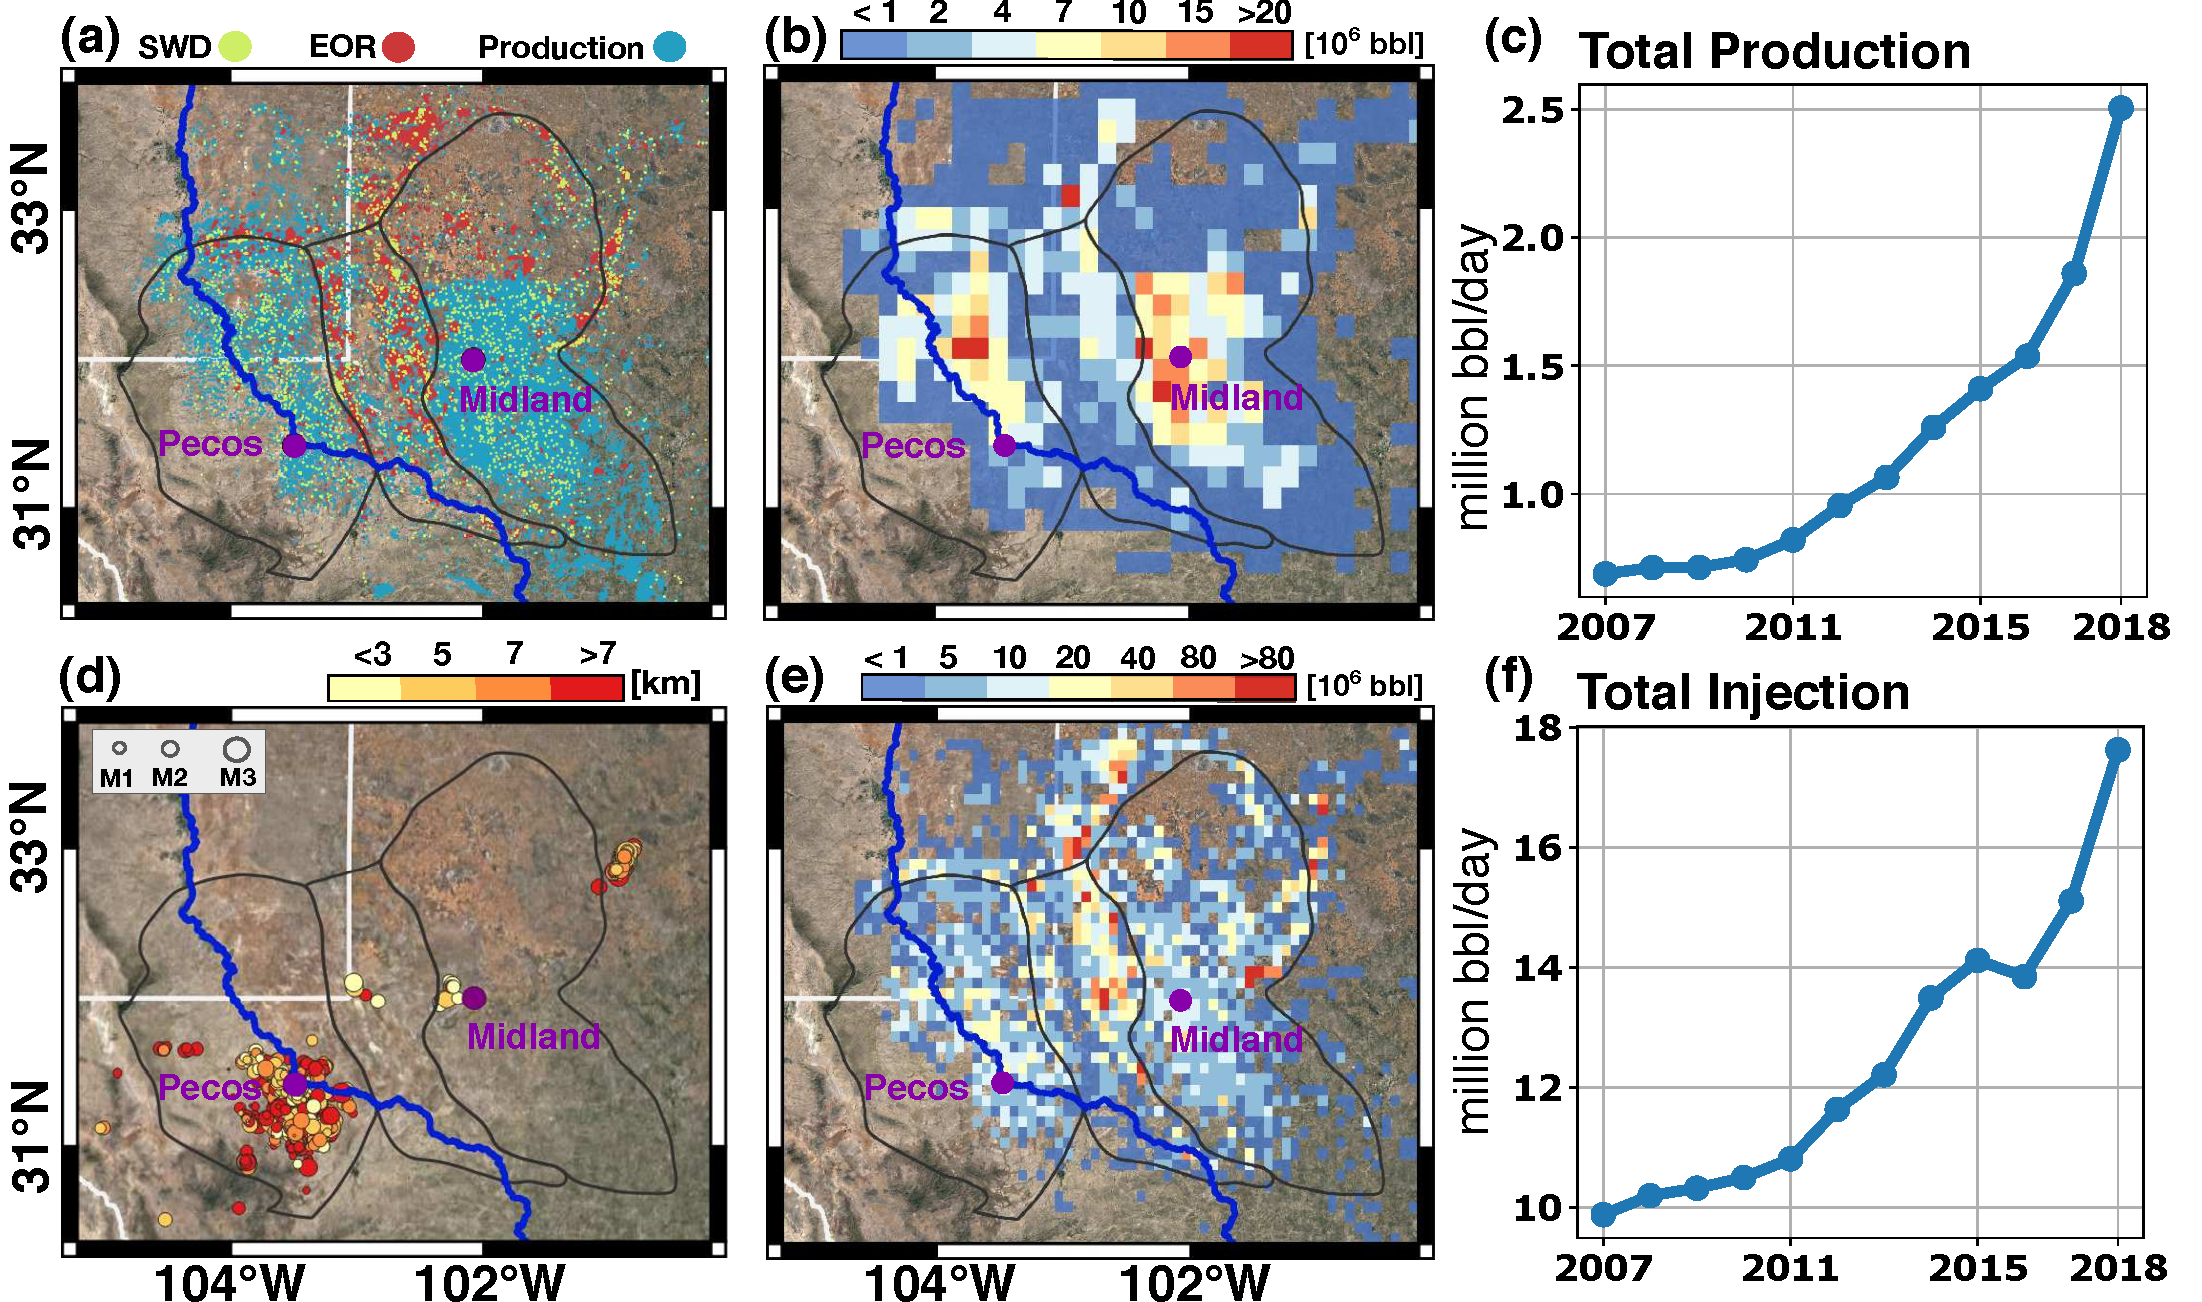
\includegraphics[width=0.99\linewidth]{figures/chapter4-grl/supplement/figureS1-cisr-data.pdf}
	\caption[Shale development and seismicity in the Permian Basin.]{Shale development and seismicity in the Permian Basin through 2018. 
		(a) Locations of oil production, EOR, and saltwater disposal (SWD) wells active in 2017. (b) Annual oil production volume on a 10-mile grid in 2017. (c) Permian Basin oil production rate as reported by the Texas Railroad Commission. (d) Locations of earthquake hypocenters detected by TexNet in 2017. The color and size of a circle indicates the estimated earthquake depth and magnitude. (e) Annual injection volume (including both SWD and EOR wells) on a 5-mile grid. (f) Permian region injection rate (including both SWD and EOR wells) as reported by the Texas Railroad Commission.
	}
	\label{fig:permian-oil-6panel}
\end{figure}





%
%%\begin{figure}[hbt!]
%\begin{figure}
%	\centering
%	%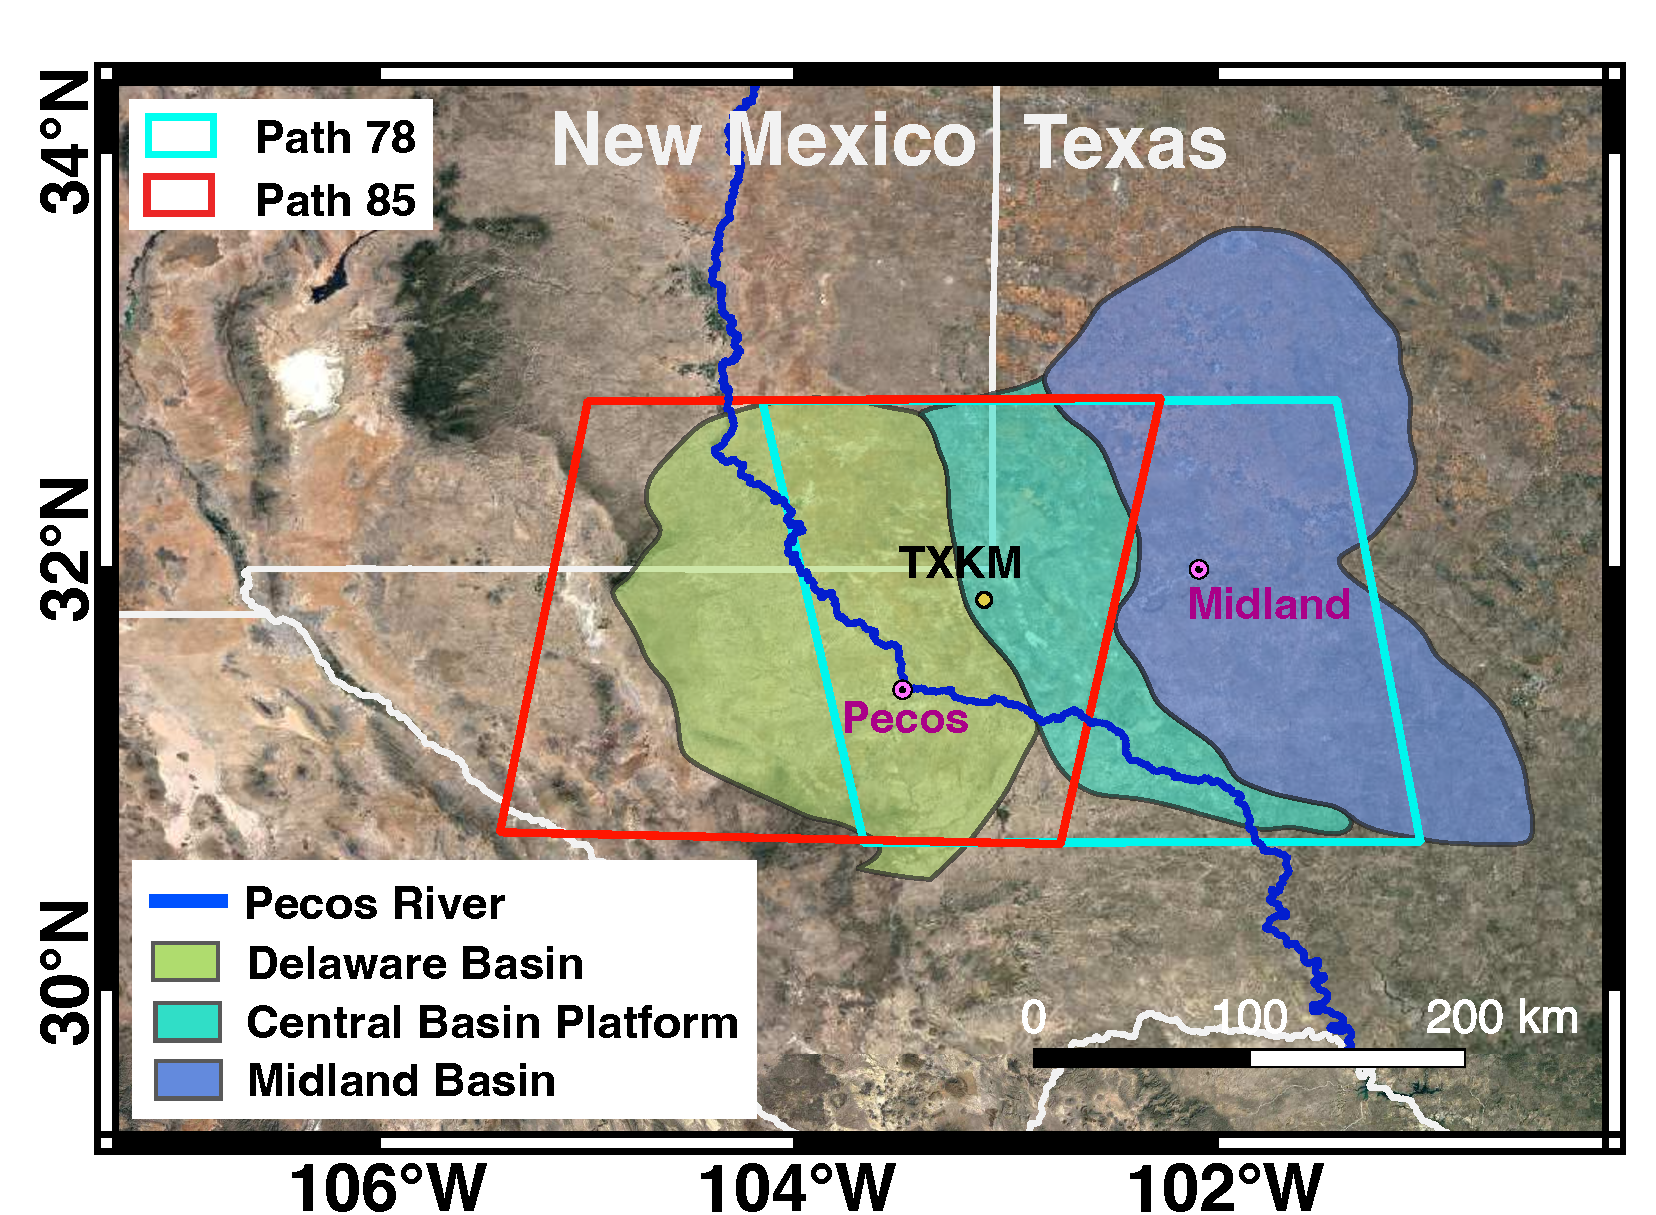
\includegraphics[width=0.9\linewidth]{figures/figure4-study-area.pdf}
%	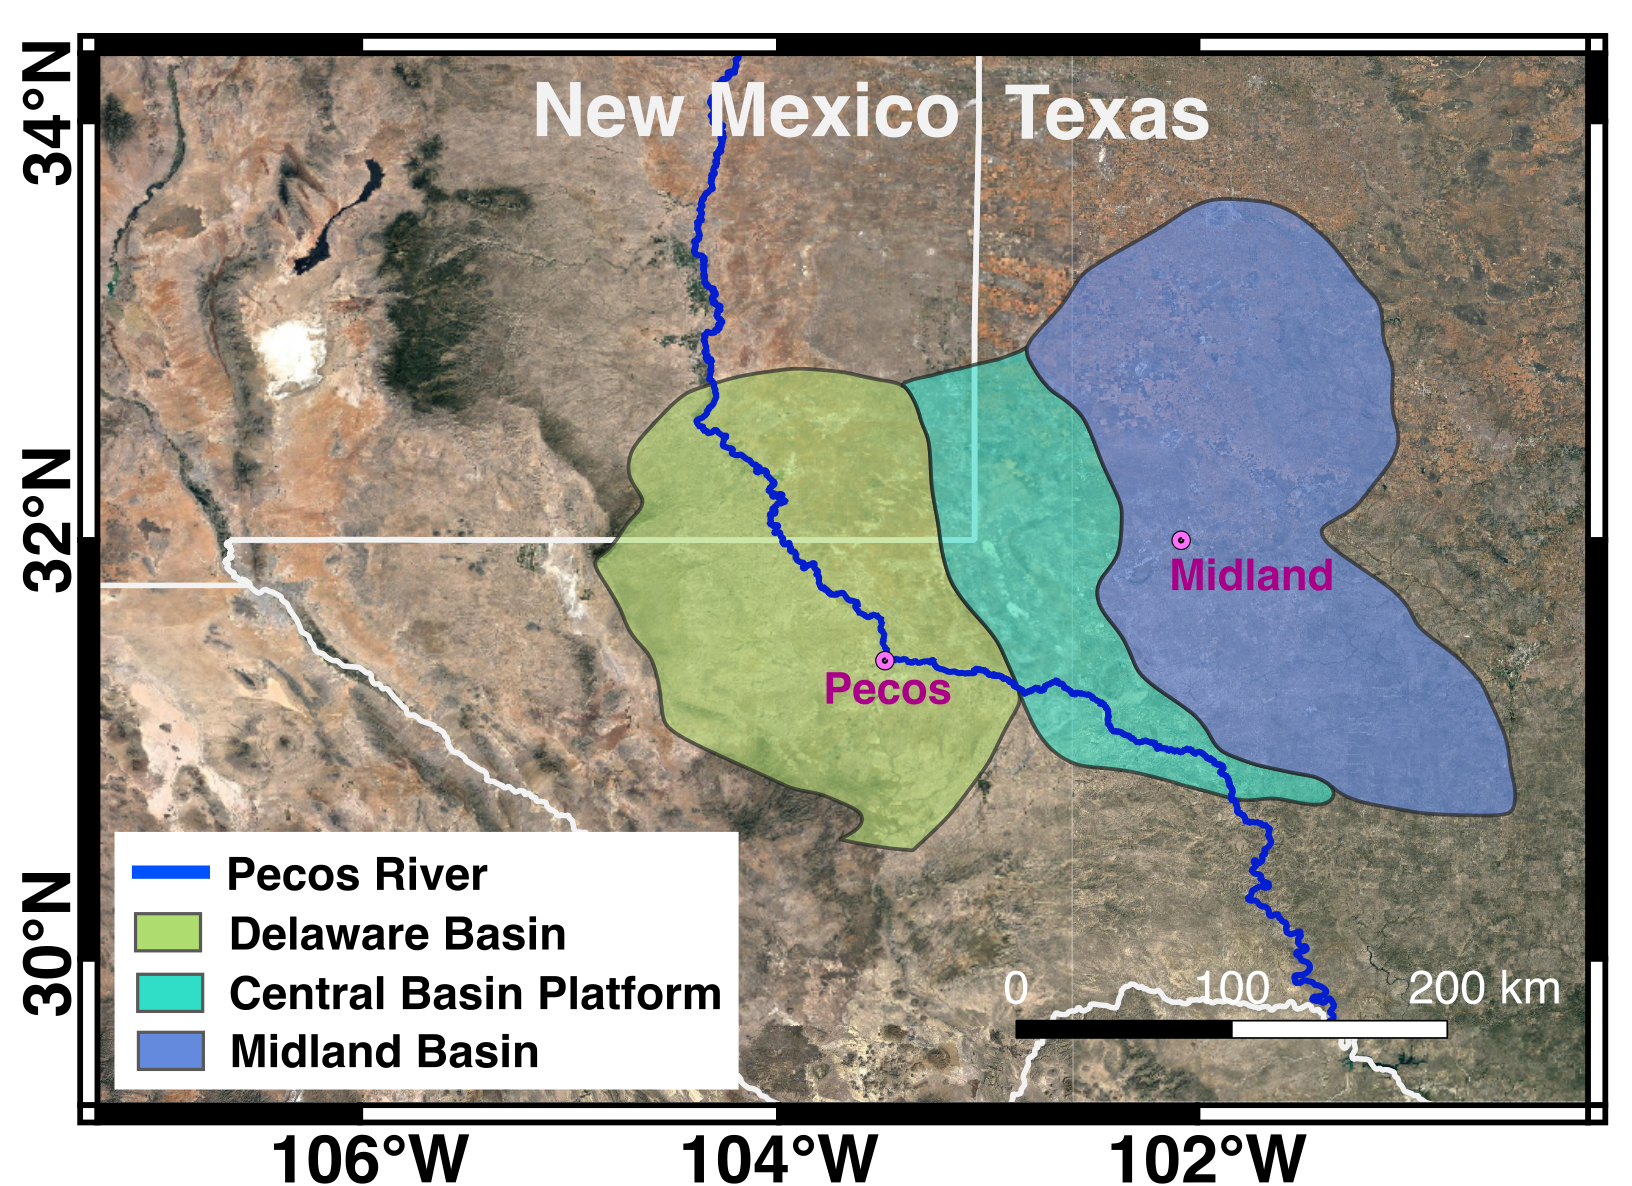
\includegraphics[width=0.96\linewidth]{figures/chapter3-permian/figure-study-area.png}
%	\caption[Subbasins within the Permian Basin]{
%		The subbasins of the Permian Basin are the Delaware Basin to the west (green) and Midland Basin to the east (purple), which are separated by the uplifed Central Basin Platform (teal).
%	}
%	\label{fig:study-area-plain}
%\end{figure}
%


% Intuitively, the spatial and temporal correlation between human activity and event occurrence may represent a key parameter to discriminate between natural and anthropogenic seismicity, but unfortunately this is not always the case. Indeed, many industrial operations involving subsurface fluid injection (e.g., wastewaterdisposal) can transmit pore pressure changes at large distance, causing earthquakes several kilometers awayfrom the industrial site.


%Attributing causation of earthquakes to individual wells may be impossible in many cases due to the proximity of many wells, but 

Several studies have used spatio-temporal analyses to link certain instances of wastewater injection and hydraulic fracturing to earthquakes \citep{Savvaidis2020InducedSeismicityDelaware, Skoumal2020InducedSeismicityDelaware, Grigoratos2020EarthquakesInducedWastewatera}, but attributing causation of earthquakes to individual wells and discriminating induced from natural seismicity is extremely challenging \citep{Grigoli2017CurrentChallengesMonitoring, Dahm2012RecommendationDiscriminationHuman, Verdon2019ImprovedFrameworkDiscriminating,Frohlich2016HistoricalReviewInduced, Frohlich2016ReplyCommentA}.
%Without a detailed study involving multiple disciplines and observational datasets, 
%Recent efforts have considerably improved the public knowledge of subsurface fault locations (Horne?), geological characterization \citep{Smye2021LithologyReservoirProperties, Smye2021VariationsVerticalStress}, pore pressure distribution and... fault system stability \citep{Hennings2021StabilityFaultSystems} 
Understanding the causes of earthquakes and how they are linked to certain production and disposal requires extensive knowledge of the subsurface.
Subsurface measurements of pore pressure changes can be difficult or impossible to collect at a regional scale, but measurements of surface deformation derived from geodetic data have been a valuable tool in estimating the distribution of fault slip at depth and inferring associated seismic risk \citep{Segall2010EarthquakeVolcanoDeformation, Huang2017FaultGeometryInversion}.


\section{Available Geodetic Data}
\label{sec:ch3-geodetic-data}

%- next: geodetic data
%- need basin wide character...
%- *check PNAS independent section*
%- first GPS: show one GPS time series
%- all look like this
%- 'for long time, assumed rigid, no deformation'
%- insar has this coverage
%- then talk processing
%- thern ' infollowing section, well see how to produce robust surface defo' (presumable revied all the challenges...)
%





%The coverage of GPS permanent stations in West Texas is sparse, and there are 14 permanent GPS stations that recorded daily east, north, and up (ENU) surface deformation measurements (Figure \ref{fig:paper1-study-area}) \citep{Blewitt2018HarnessingGpsData}. After removing the common tectonic motion, all GPS stations showed little surface deformation (0-3 mm/year) between Nov. 2014 and Jan. 2019.

The coverage of GPS permanent stations in West Texas is sparse, and there are no stations in the Delaware Basin (Figure \ref{fig:paper1-study-area}). At 14 stations in the Midland Basin and the Central Basin Platform, daily east, north, and up (ENU) surface deformation measurements were processed by the Nevada Geodetic Laboratory \citep{Blewitt2018HarnessingGpsData}. After removing the regional tectonic motion, little motion (0-3 mm/year) was observed at all GPS stations over the study period (Figure \ref{fig:ch3-gps}). Because energy-related injection and extraction activities often occur within deep and rigid subsurface formations, it has been common to assume little deformation can be detected at Earth's surface. 
%Thus, the available permanent GPS stations are too sparse to provide a full picture of surface changes, 


InSAR surface deformation measurements have much broader spatial coverage, and they provide a key observable to fill the gaps left by GPS. They allow us to estimate locations of pressure build up from fluid injection, barriers to subsurface fluid flow, and unmapped faults. However, creating accurate maps of surface deformation using InSAR can be challenging at the scale of the full Permian Basin.

\begin{figure}
	\centering
	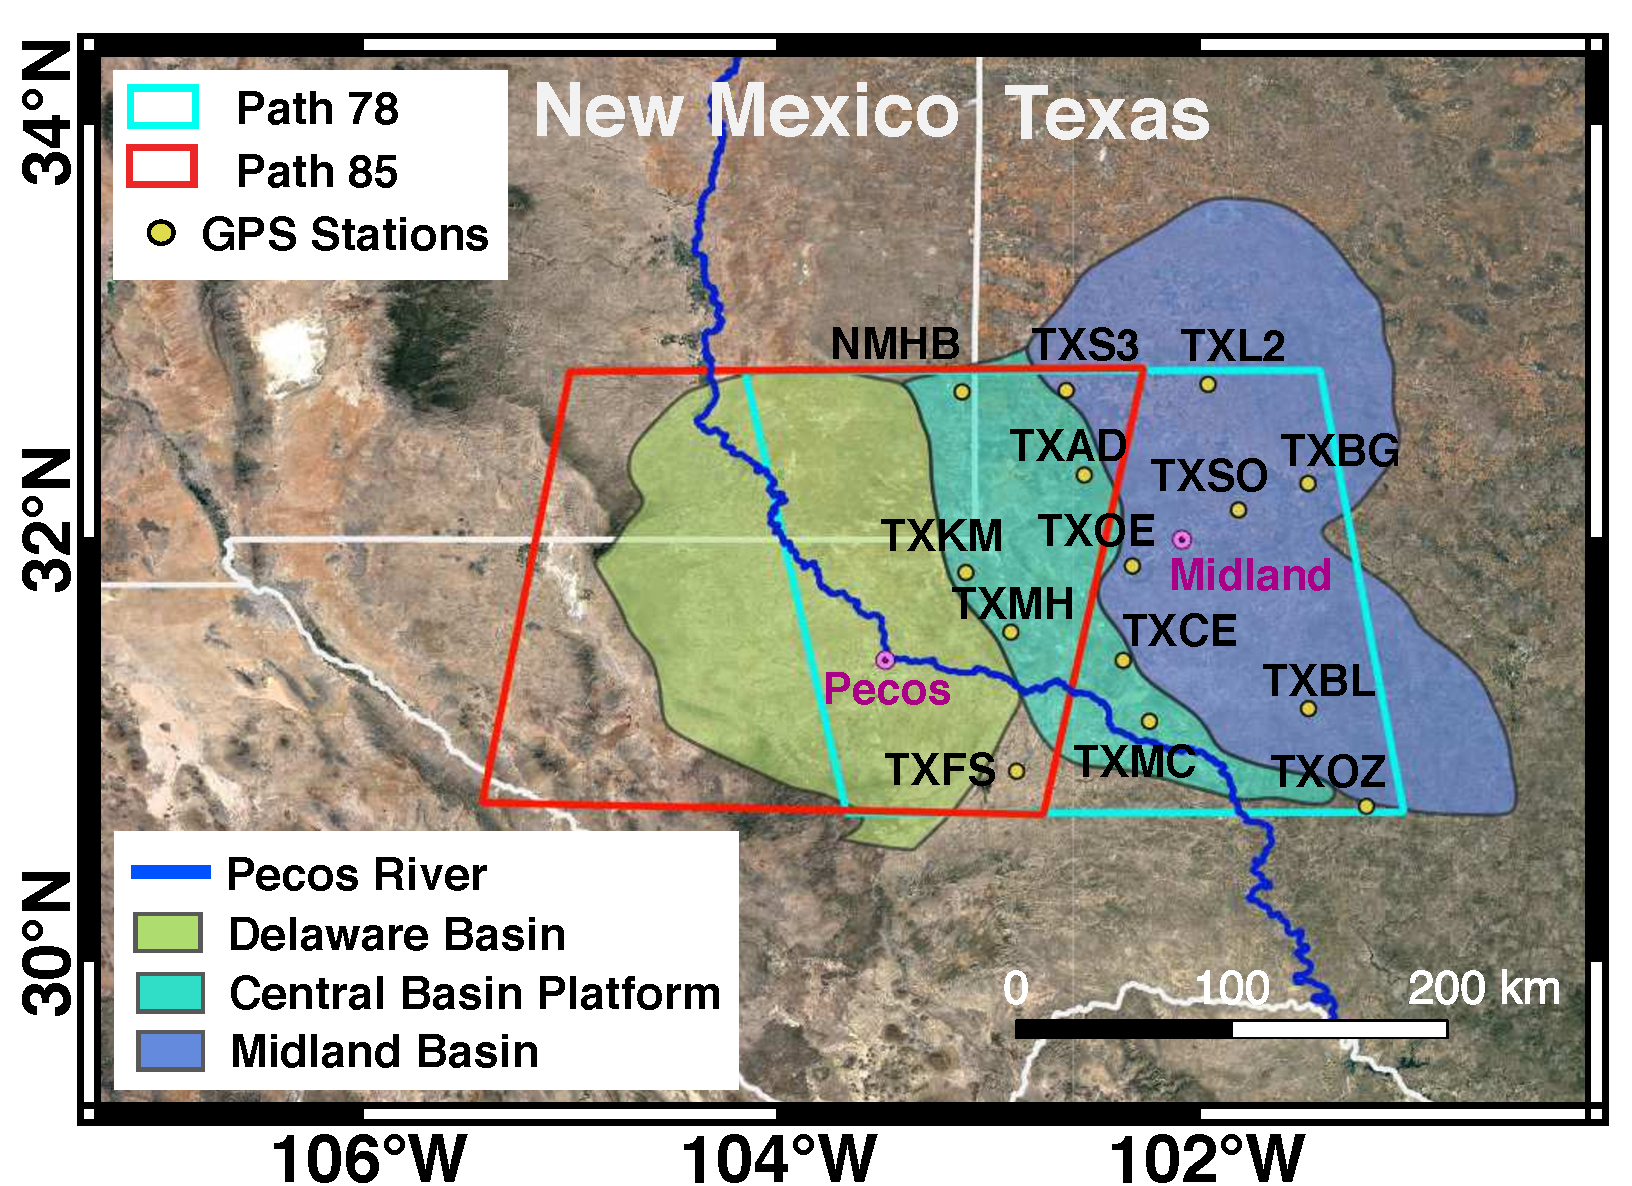
\includegraphics[width=0.9\linewidth]{figures/chapter4-grl/figure1-study-area.pdf}
	\caption[GPS and InSAR data coverage over the Permian Basin.]{GPS and InSAR data coverage over the Permian Basin. Yellow dots indicate GPS permanent stations. Teal and red boxes indicate ascending path 78 and descending path 85 paths of Sentinel 1 InSAR coverage, respectively. 
		%	Each path contains over 80 SAR acquisitions, leading to over 3500 interferograms per path at 120 m pixel spacing.
	}
	\label{fig:paper1-study-area}
\end{figure}

\begin{figure}
	\centering
	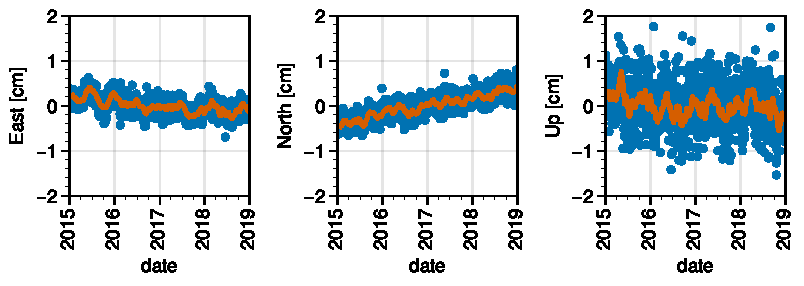
\includegraphics[width=0.99\linewidth]{figures/chapter3-permian/gps-txmc.pdf}
	\caption[Example permanent GPS station measurements]{
		Example measurements of east, north, and vertical components of surface deformation from the permanent GPS station TXMC (Figure \ref{fig:paper1-study-area}). All stations indicated in Figure \ref{fig:paper1-study-area} show similarly small deformation during the 2015-2019 period.
	}
	\label{fig:ch3-gps}
\end{figure}


\FloatBarrier

\section{InSAR Processing Strategy and Noise Assessment}
\label{sec:ch3-insar-processing}

Using a geocoded SLC processor \citep{Zheng2017PhaseCorrectionSingle, Zebker2017UserFriendlyInsar} (Section \ref{sec:ch2-processing}), we processed 91 ascending (path 78, frames 94-104) and 82 descending (path 85, frames 483-493) Sentinel-1 scenes acquired between Nov. 2014 and Jan. 2019 (Figure \ref{fig:paper1-study-area}). We generated more than 7000 interferograms with 120 meter pixel spacing and a maximum temporal baseline of 800 days. No spatial baseline threshold was imposed in the interferogram formation. Because few decorrelation artifacts were present, we were able to unwrap all interferograms without additional spatial filtering using the Statistical-cost, Network-flow Algorithm for Phase Unwrapping (SNAPHU) \citep{Chen2001TwoDimensionalPhase}. We removed long-wavelength phase ramps due tropospheric noise using a planar phase model.
We chose the GPS station TXKM as the reference point for both ascending and descending InSAR data, and we used the remaining 13 stations as controls to assess InSAR measurement uncertainty (Chapter \ref{CHAP:4-GRL}).
Comparable interferograms can be generated using other processors such as the InSAR Scientific Computing Environment (ISCE) \citep{Rosen2012InsarScientificComputing} or GMTSAR \citep{Sandwell2011OpenRadarInterferometry}. 

Interferograms may contain noise from many possible sources (Section \ref{sec:ch2-noise}). %orbital errors, phase decorrelation, unwrapping errors, DEM inaccuracies, ionospheric and tropospheric artifacts, and other residual noise terms. 
In our West Texas data, $\Delta \phi_{orb}$ was negligible, and interferograms containing significant decorrelation, $\Delta \phi_{decor}$, or unwrapping artifacts, $\Delta \phi_{unwrap}$, were removed. Because the Permian Basin is located in the middle latitudes and is relatively flat, $\Delta \phi_{iono}$ and $\Delta \phi_{dem}$  are not substantial \citep{Fattahi2013DemErrorCorrection, Liang2019IonosphericCorrectionInsar}. 
Tropospheric noise $\Delta \phi_{tropo}$ consists of a stratified component that correlates with topography \citep{Doin2009CorrectionsStratifiedTropospheric} and a turbulent component that is random at time scales longer than one day \citep{Emardson2003NeutralAtmosphericDelay} (Section \ref{sec:ch2-noise-tropo}).
Since the majority of the oil-producing Permian Basin is flat (less than 700 meters of elevation change), there is not a substantial stratified component of tropospheric noise in our data. 
The dominant noise source in the West Texas Sentinel-1 data is turbulent tropospheric noise.
%For the reminder of this section, we focused on evaluating and mitigating the impact of tropospheric noise on the West Texas Sentinel-1 data.


%I also think it is much easier to first state, the study area is flat, and thus there is no substantial stratified tropospheric noise component. Then explain why GACOS does not work (no dense GPS network, and the weather models mainly capture the stratified component). This is a good place to include your GRL Supp on GACOS figure for the Permian Basin correction results (You may have mentioned GACOS in the radar section, but the discussion there should be more general without specific West Texas results).

%This is because the oil-producing region of the Permian Basin is relatively flat, and we observed little correlation between InSAR LOS measurements and the Digital Elevation Model (DEM) data 
%(see Section \ref{sec:ch3-noise-tropo-mitigate}).


We analyzed the effectiveness of tropospheric correction techniques based on auxiliary data using the Generic Atmospheric Correction Online Service (GACOS, \citep{Yu2018InterferometricSyntheticAperture,Yu2018GenericAtmosphericCorrection}), 
which derives its corrections using the High Resolution European Centre for Medium-Range Weather Forecasts (ECMWF) weather model (0.125-degree, 6-hour resolutions) and the GNSS-derived zenith delay maps from the Nevada Geodetic Laboratory.
%which combines global atmospheric models (GAMs) and GPS data to produce synthetic delay maps. 
%GACOS derives its corrections using the High Resolution European Centre for Medium-Range Weather Forecasts (ECMWF) weather model (0.125-degree, 6-hour resolutions) and the GNSS derived tropospheric delay products from Nevada Geodetic Laboratory.
Note that for the West Texas region, GACOS mostly relies on the weather model input due to the sparsity of GPS stations.


%Due to the limited spatial and temporal resolution of weather models and GPS data, GACOS is more effective in removing the stratified tropospheric noise \citep{Doin2009CorrectionsStratifiedTropospheric} than the random turbulent tropospheric noise \citep{Emardson2003NeutralAtmosphericDelay}. 
%We found that GACOS does not produce substantial corrections in most Sentinel-1 West Texas interferograms for areas outside the main area of interest (e.g. Figure \ref{fig:GACOS} (a)-(c)).


%% RMS REDUCTIONS %%
%WAVE: Before6.45, after: 3.45 cm RMS. Reduction of 46.5%
% STORM: Before3.34, after: 3.24 cm RMS. Reduction of 2.9%
%
%RMS: (before, after)
%datepair='20150127_20150220':
%RMS: 4.06, 2.41
%datepair='20150515_20150726':
%RMS: 2.92, 1.91
%datepair='20150304_20150328':
%RMS: 2.12, 1.23
%datepair='20150608_20150702':
%RMS: 2.61, 4.44
%datepair='20150127_20150304':
%RMS: 3.83, 2.09



\begin{figure}
	\centering
	%	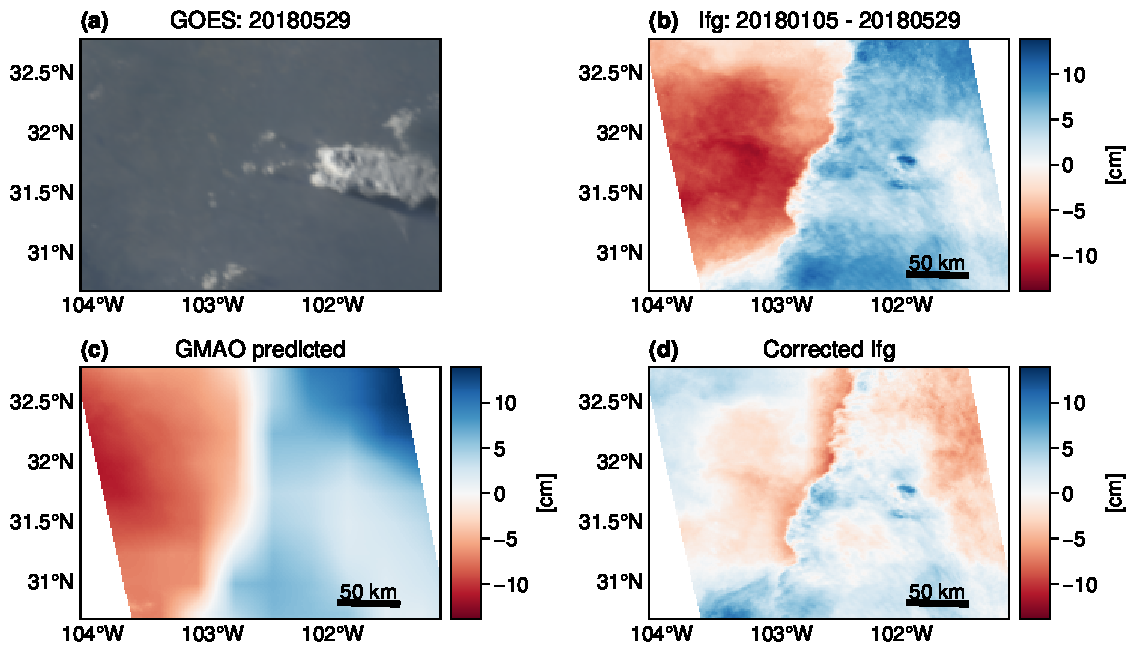
\includegraphics[width=1.0\textwidth]{figures/chapter2-sar/figure_tropo_correct_wave.pdf}
	%	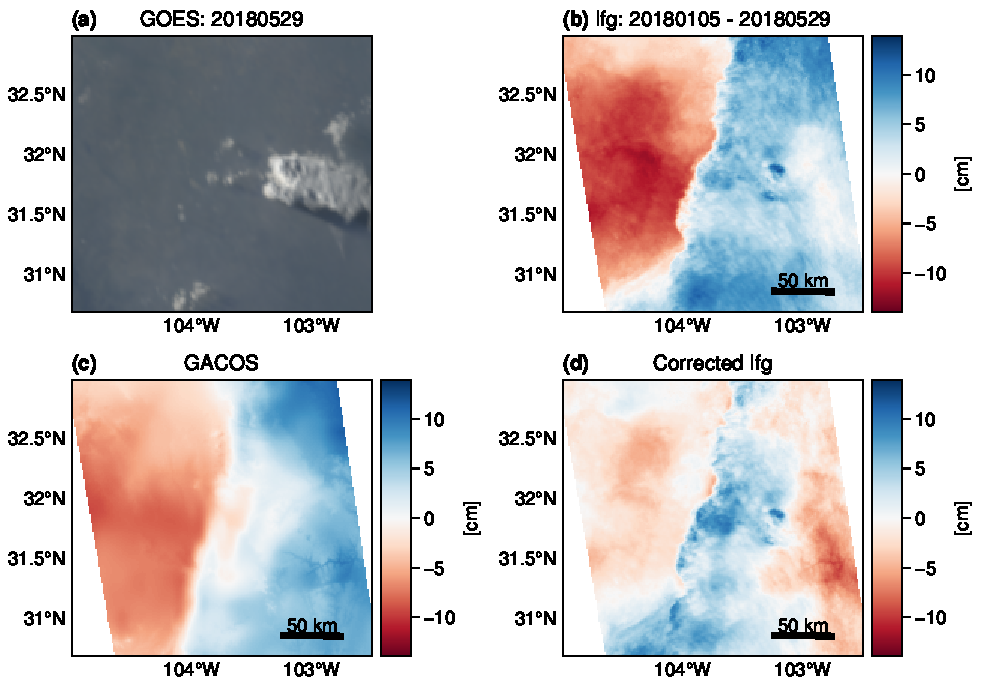
\includegraphics[width=1.0\textwidth]{figures/chapter2-sar/figure_tropo_correct_gacos_wave.pdf}
	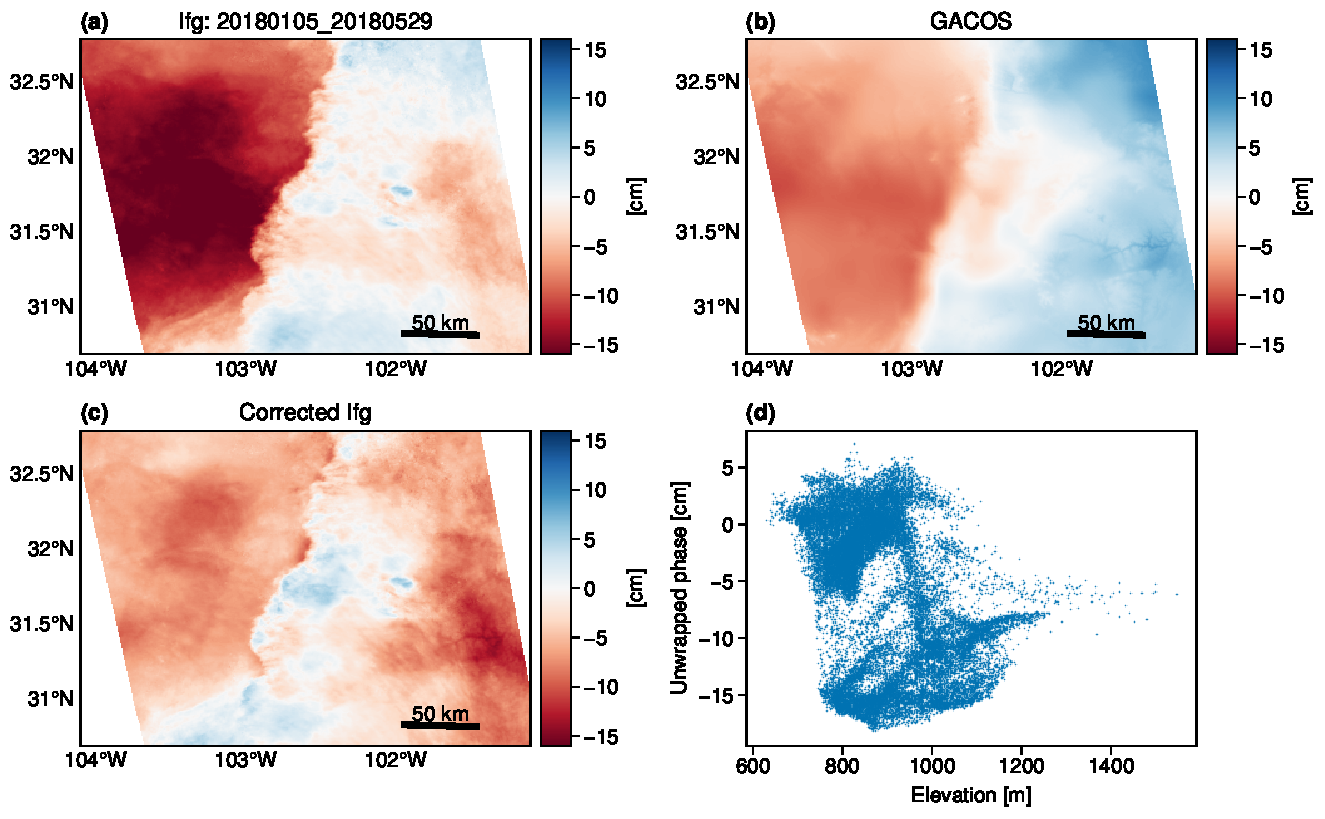
\includegraphics[width=1.0\textwidth]{figures/chapter2-sar/figure_tropo_correct_gacos_wave_ph_vs_el.pdf}
	\caption[West Texas tropospheric correction for interferogram containing weather front]{
%		(a) Weather conditions visible from the GOES satellite on May 29th, 2018 at the same time as the Sentinel-1 acquisition.
		(a) Unwrapped interferogram from Jan. 5, 2018 to May 29, 2018. Blue indicates an increase in relative LOS delay.
		(b) Tropospheric correction predicted from delays computed by GACOS.
		(c) Corrected interferogram (panel (b) - panel (c))
		(d) Unwrapped LOS measurements (in cm) of the 20180105-20180529 interferogram vs. the Digital Elevation Model (DEM) heights.
	}
	\label{fig:ch2-tropo-correct-wave}
\end{figure}



%We illustrate two correction attempts for Sentinel-1 (path 78) interferograms over West Texas using GAM-based corrections produced by RAiDER (Figures \ref{fig:ch2-tropo-correct-wave},\ref{fig:ch2-tropo-correct-storm}). We use NASA's Global Modeling and Assimilation Office (GMAO) reanalysis weather models, which are interpolated by RAiDER to the same pixel spacing as the interferograms ($\sim$ 500 m for this example). 
We illustrate several correction attempts for Sentinel-1 interferograms over West Texas using GACOS tropospheric corrections.
% (Figures \ref{fig:ch2-tropo-correct-wave},\ref{fig:ch2-tropo-correct-storm}). 
In Figures \ref{fig:ch2-tropo-correct-wave}, an ascending (Path 78) interferogram from Jan. 5, 2018 to May 29, 2018 contains a mass of dry air moving in from the New Mexico mountains, which creates a $\sim 20$ cm decrease in LOS delay in half of the interferogram (Figure \ref{fig:ch2-tropo-correct-wave}a, red).
Here the ECMWF weather model used by GACOS predicts the some of the delay change between the dates Figure \ref{fig:ch2-tropo-correct-wave}b). 
The root mean square (RMS) noise drops from 8.8 cm in the original interferogram to 5.7 cm after the GACOS correction (Figure \ref{fig:ch2-tropo-correct-wave}c), despite the interferogram showing no discernible phase vs. elevation trend (Figure \ref{fig:ch2-tropo-correct-wave}d). 

 
In other examples, the GACOS corrections provided little benefit, and occasionally added noise to the interferogram. For example, Figure \ref{fig:ch2-tropo-correct-gacos-fail}a shows a descending Path 85 interferogram from June 8, 2015 to July 2, 2015. The GACOS correction is not correlated with the interferogram noise structure (Figure \ref{fig:ch2-tropo-correct-gacos-fail}b), and the RMS noise in the corrected interferogram (Figure \ref{fig:ch2-tropo-correct-gacos-fail}c) increased from 2.6 cm to 2.9 cm.


\begin{figure}
	\centering
	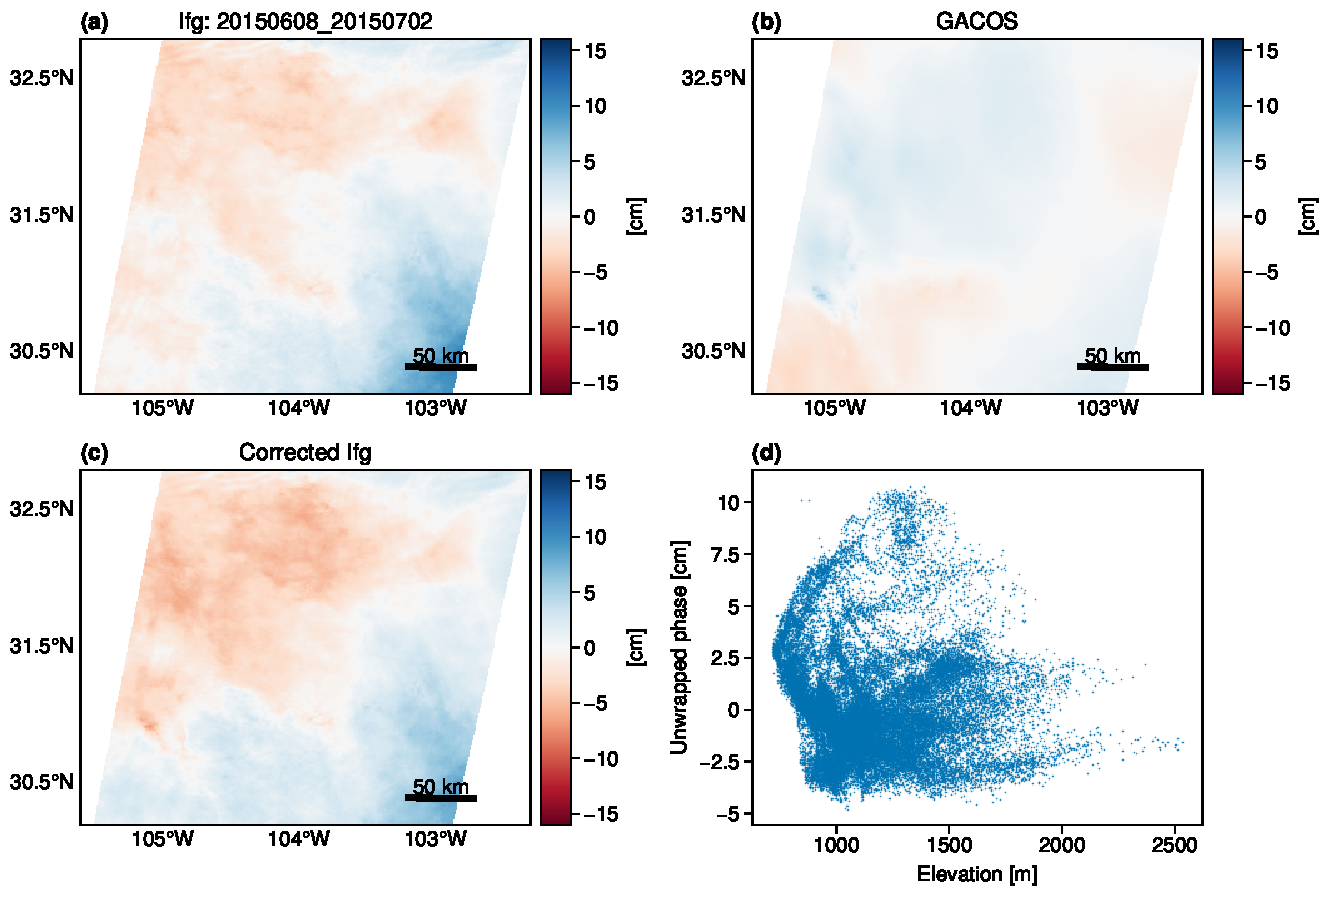
\includegraphics[width=1.0\textwidth]{figures/chapter2-sar/figure_tropo_correct_gacos_20150608_20150702.pdf}
	\caption[GACOS tropospheric correction attempt on descending interferogram]{
		(a) Descending Path 85 unwrapped interferogram from June 8, 2015 to July. 2, 2015. Blue indicates an increase in relative LOS delay
		(b) Tropospheric correction predicted from delays computed by GACOS.
		(c) Corrected interferogram (panel (a) - panel (b))
		(d) Unwrapped LOS measurements (in cm) of the 20150608-20150702 interferogram vs. the Digital Elevation Model (DEM) heights.
	}
	\label{fig:ch2-tropo-correct-gacos-fail}
\end{figure}

%We also compare the weather conditions that are visible at the secondary SAR acquisition time using the Geostationary Operational Environmental Satellites (GOES).
\FloatBarrier

Thunderstorms commonly add 10-15 cm of turbulent tropospheric noise to interferograms using a summer SAR acquisition (Figure \ref{fig:ch2-tropo-correct-storm}).
During summer months, the weather conditions at the SAR acquisition time are visible in optical images taken by the Geostationary Operational Environmental Satellites (GOES) (Figure \ref{fig:ch2-tropo-correct-storm}a).
%For both Figures \ref{fig:ch2-tropo-correct-wave}, \ref{fig:ch2-tropo-correct-storm}, the earlier SAR acquisition occurs during winter, which is after sunset for ascending Sentinel-1 over West Texas. Most of the tropospheric noise in these winter-to-summer interferograms comes from the summer SAR acquisition.
%The first example contains strong tropospheric noise resulting from a mass of dry air moving in from the New Mexico mountains, which creates a $\sim 20$ cm decrease in LOS delay in half of the interferogram (Figure \ref{fig:ch2-tropo-correct-wave}b). This change is not visible in the optical GOES image (Figure \ref{fig:ch2-tropo-correct-wave}a), but is predicted in the global weather model (Figure \ref{fig:ch2-tropo-correct-wave}c). 
%The root mean square (RMS) noise drops from 6.4 cm in the original interferogram to 3.5 cm after the GACOS correction.
%, the slight temporal differences of the model output and interferogram acquisition times lead to only a partial correction of the tropospheric pattern.
%Although the root mean square (RMS) noise of the corrected interferogram drops from 6.4 cm to 2.8 cm, the slight temporal differences of the model output and interferogram acquisition times lead to only a partial correction of the tropospheric pattern.
%		(a) Weather conditions visible from the GOES satellite on July 23rd, 2019 at the same time as the Sentinel-1 acquisition
For example, tall cumulonimbus clouds covered much of West Texas on July 23, 2019 at the time of the Sentinel-1 acquisition (Figure \ref{fig:ch2-tropo-correct-storm}a), which created patches of excess delay of $>10$ cm in the interferogram from Jan. 12 to July 23, 2019 (Figure \ref{fig:ch2-tropo-correct-storm}b).
The different imaging geometries of the Sentinel-1 satellites (side-looking, in low Earth orbit) and the GOES satellites (nadir-looking, geostationary orbit) mean the pixels of Figure \ref{fig:ch2-tropo-correct-storm}a and Figure \ref{fig:ch2-tropo-correct-storm}b do not fully align, but cover approximately the same area.
The $\sim 5$ km storm cells are not predicted by GACOS due to the relatively coarse spatial and temporal resolution of global weather models (Figure \ref{fig:ch2-tropo-correct-storm}c). Thus, the corrected interferogram still contains most of the turbulent noise from the storm (Figure \ref{fig:ch2-tropo-correct-storm}d).


\begin{figure}
	\centering
%	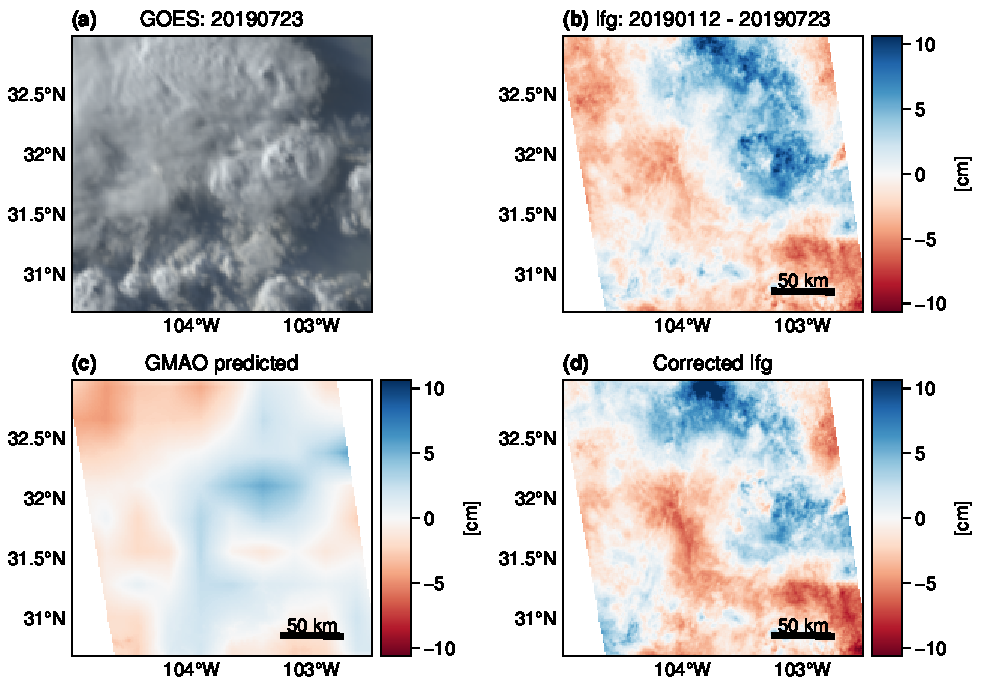
\includegraphics[width=1.0\textwidth]{figures/chapter2-sar/figure_tropo_correct_storm.pdf}
	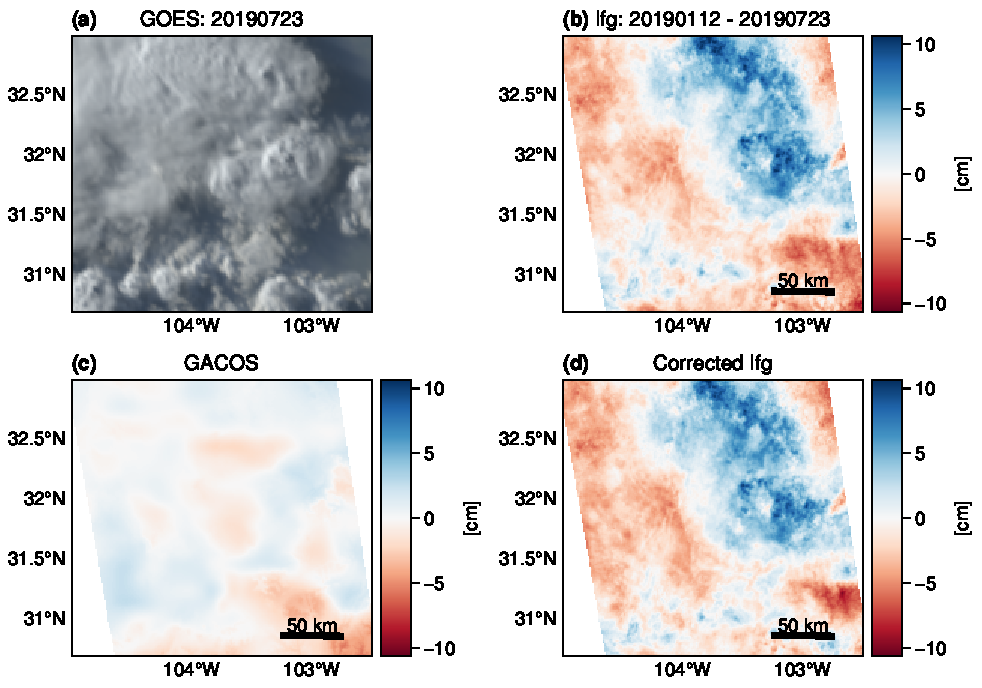
\includegraphics[width=1.0\textwidth]{figures/chapter2-sar/figure_tropo_correct_gacos_storm.pdf}	
	\caption[West Texas tropospheric correction attempt for thunderstorm]{
		(a) Weather conditions visible from the GOES satellite on July 23rd, 2019 at the same time as the Sentinel-1 acquisition
		(b) Unwrapped interferogram from Jan. 12, 2019 to July 23, 2019. Blue indicates an increase in relative LOS delay
		(c) Tropospheric correction predicted from delays computed by GACOS.
		(d) Corrected interferogram (panel (b) - panel (c))
	}
	\label{fig:ch2-tropo-correct-storm}
\end{figure}

%\begin{figure}
%	\centering
%%	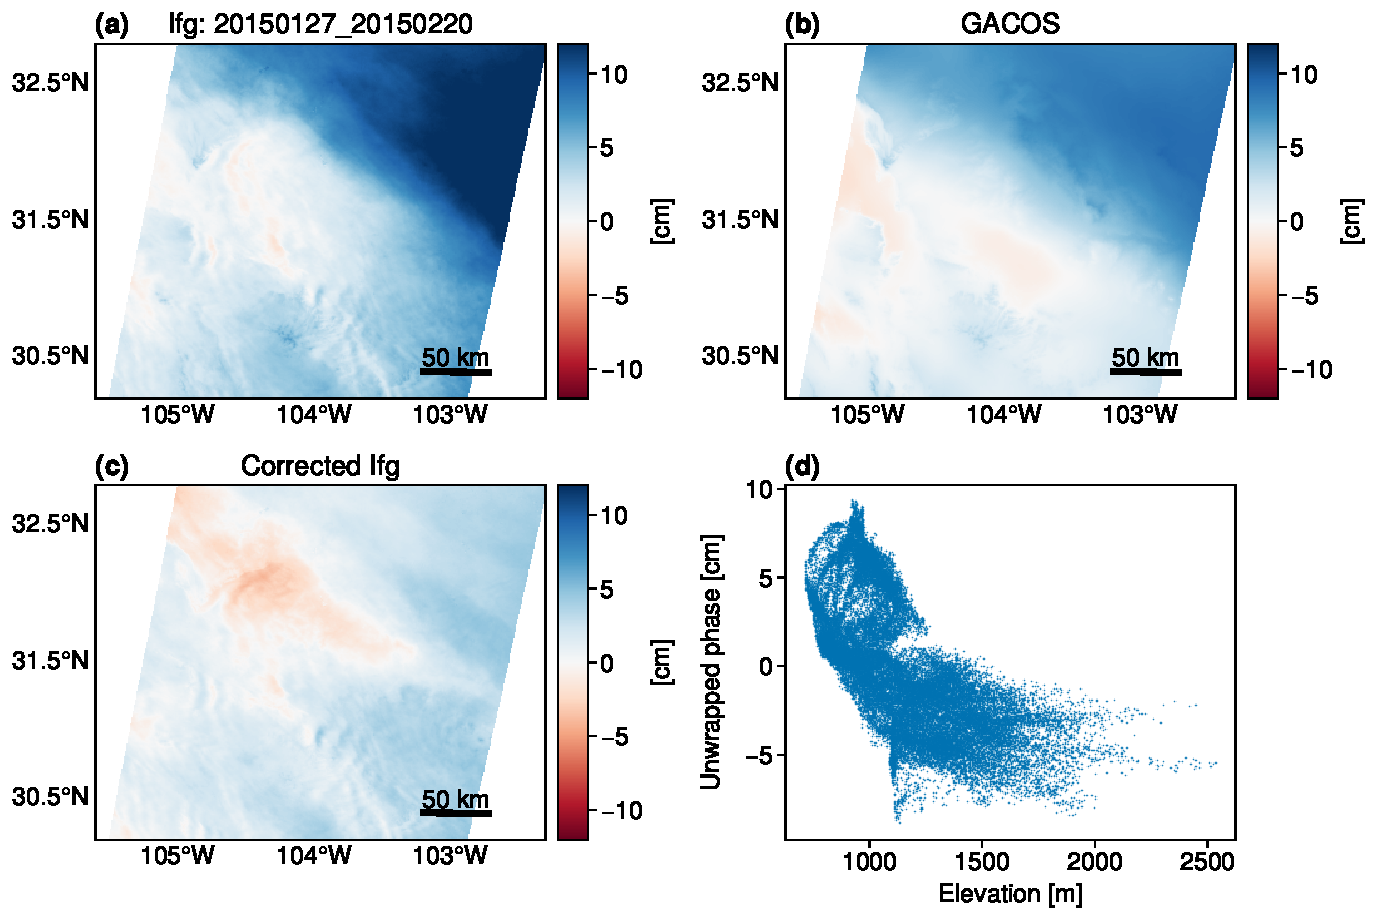
\includegraphics[width=1.0\textwidth]{figures/chapter2-sar/figure_tropo_correct_gacos_20150127_20150220.pdf}
%	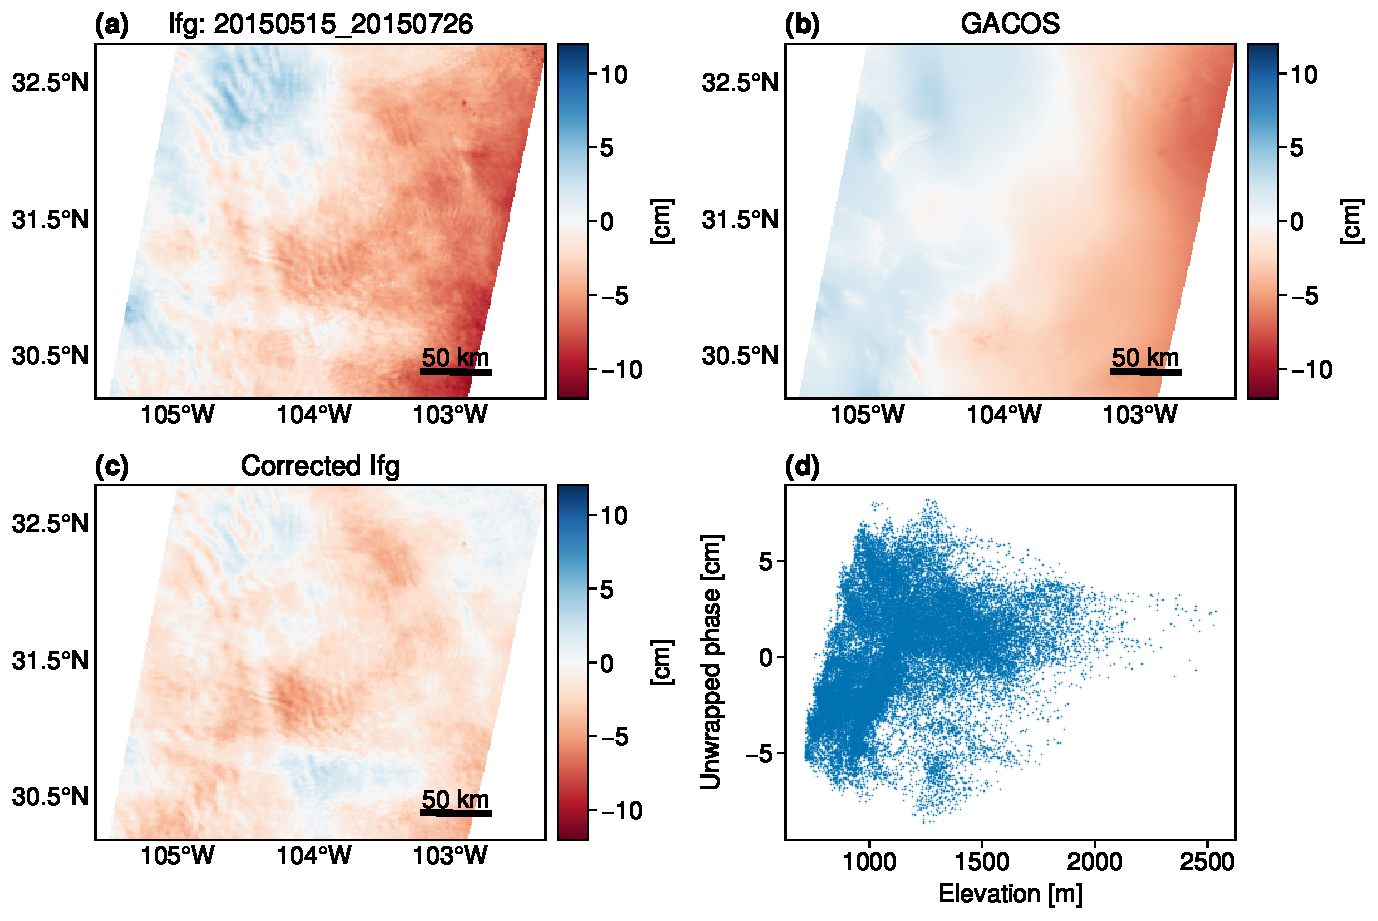
\includegraphics[width=1.0\textwidth]{figures/chapter2-sar/figure_tropo_correct_gacos_20150515_20150726.pdf}
%	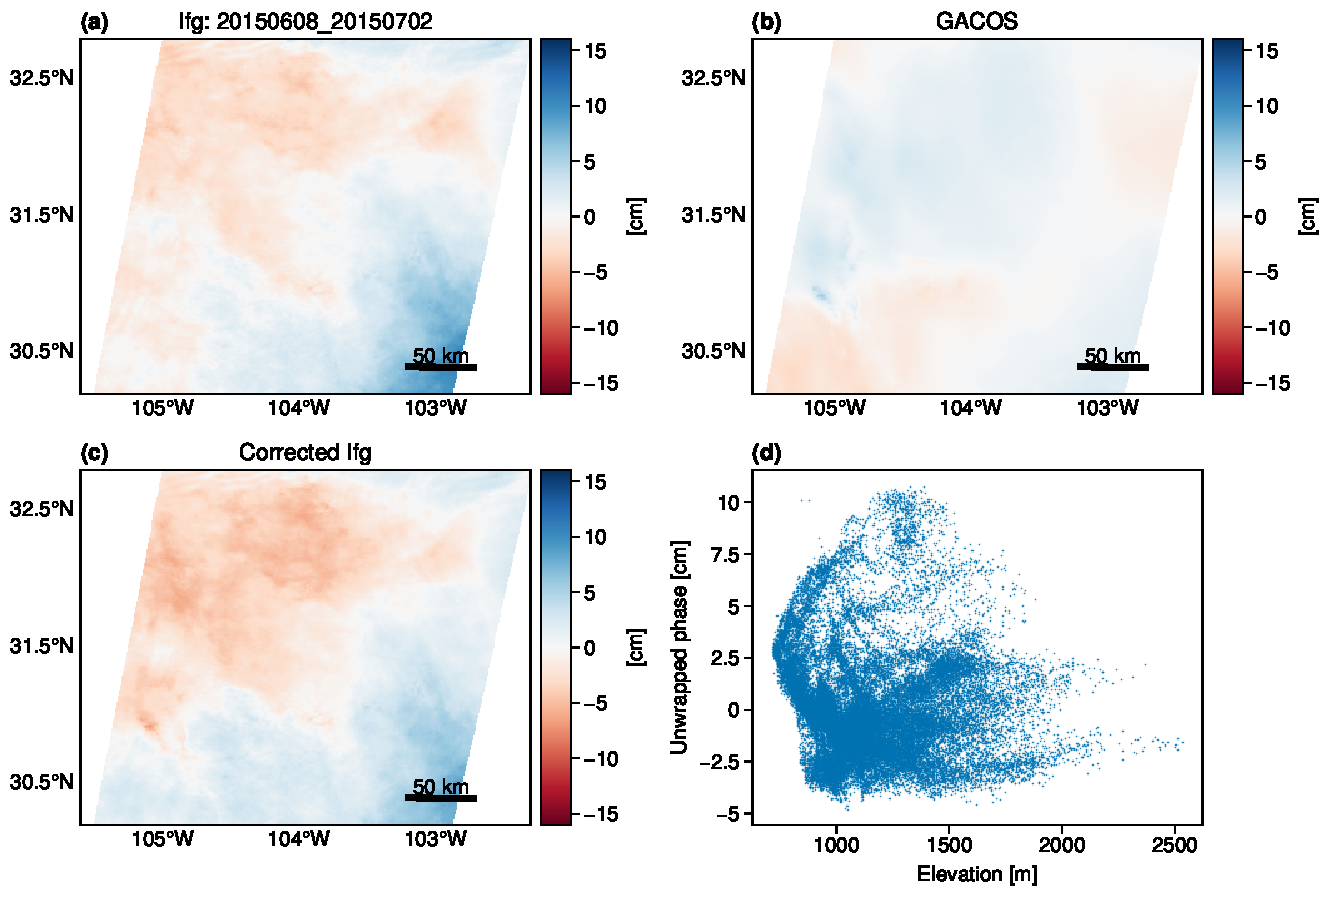
\includegraphics[width=1.0\textwidth]{figures/chapter2-sar/figure_tropo_correct_gacos_20150608_20150702.pdf}
%	\caption[West Texas tropospheric correction attempt for thunderstorm]{
%		(a) Weather conditions visible from the GOES satellite on July 23rd, 2019 at the same time as the Sentinel-1 acquisition
%		(b) Unwrapped interferogram from Jan. 12, 2019 to July 23, 2019. Blue indicates an increase in relative LOS delay
%		(c) Tropospheric correction predicted from delays computed by GACOS.
%		(d) Corrected interferogram (panel (b) - panel (c))
%	}
%	\label{fig:ch2-tropo-correct-storm}
%\end{figure}


We also created line-of-sight delay estimates from weather models using the Raytracing Atmospheric Delay Estimation for Radar (RAiDER) library of \cite{Maurer2021RaiderRaytracingAtmospheric}. RAiDER generates a troposphere correction product by integrating the model-predicted delay along the radar LOS path for each InSAR pixel. We compared several weather model corrections to the ECMWF used by GACOS and found only small differences in the results. For example, the RMS noise of the interferogram in Figure \ref{fig:ch2-tropo-correct-wave} drops an additional 0.8 cm by using NASA's Global Modeling and Assimilation Office (GMAO) reanalysis weather model, despite have 5x coarser spatial resolution than the ECMWF. However, no model that we tested successfully generated corrections for Figure \ref{fig:ch2-tropo-correct-storm}.

 
%The dominant noise term for our West Texas Sentinel-1 data is turbulenct tropospheric noise.
Since the turbulent tropospheric noise is difficult to predict and correct using the auxiliary correction methods, Chapters \ref{CHAP:4-GRL} and \ref{CHAP:5-robust-ts} present data-driven mitigation strategies for producing robust estimates of surface deformation.



